%===================================================================================
% Chapter: Análisis Experimental
%===================================================================================
\chapter{Análisis Experimental}\label{chapter:experiments}
\addcontentsline{toc}{chapter}{Análisis Experimental}

Este capítulo se centra en la descripción del los detalles de la implementación de las propuestas descritas para la extracción de entidades y relaciones.
Se explican las configuraciones de los exprimentos realizados y el conjunto de técnicas experimentales empleadas, se muestran los resultados de dicho estudio y se someten los mismo a una posterior discusión.

\section{Marco Experimental}

El desarrollo de los experimentos de este trabajo se enmarca en el evento \textit{eHealth Knowledge Discovery Challenge}, en sus ediciones de 2019 y 2020.
En la misma, los problemas de extracción de entidades y relaciones están organizados en dos tareas.

\begin{description}
	\item[Tarea A:] Extracción y clasificación de entidades.
	Es objetivo de esta tares es, dada una lista de documentos~(oraciones) en idioma Español con contenido médico, extraer las entidades relevantes presentes en dicho documento, y clasificarlas de acuerdo al tipo de concepto que representan~(\texttt{Concept}, \texttt{Action}, \texttt{Predicate} o \texttt{Reference}).
	Las entidades son conceptos semánticamente importantes dentro de una oración.
	Pueden estar formadas por una o varias palabras, las cuales no necesariamente aparecen de manera continua en el texto de la oración.
	La figura \ref{fig:entites_ex} muestra las entidades relevantes que aparecen en un conjunto de oraciones de ejemplo.
	
	La entrada de la Tarea A es un documento de texto con una oración	por línea.
	La salida es una colección de entidades, con un identificador numérico asociado a cada una.
	Cada entidad esta constituída por una lista de segmentos del texto \texttt{<inicio, fin>}, que representan las palabras por las que está conformado dicho concepto.
	
	\item[Tarea B:] Extracción de relaciones.
	La Tarea B parte del conjunto de entidades obtenido en la Tarea A.
	El objetivo de esta tarea es indentificar las relaciones semánticas relevantes entre los conceptos encontrados en cada oración.
	Ocho de las trece relaciones semánticas presentes en los conjuntos de datos pueden ser observadas en la figura \ref{fig:relations_ex}.
		
	La entrada de la Tarea B es un documento de texto con una oración	por línea, y una colección de entidades, con su correspondiente identificador numérico y etiqueta.
	La salida de la Tarea B es una lista de tuplas de la forma \texttt{<id1,id2,rel>} que denota la existencia de una relación con origen en la entidad con identificador \texttt{id1}, y destino en \texttt{id2}, y que se le asigna el tipo \texttt{rel}.
	
\end{description} 
	
\begin{figure}[h!]
	\centering
	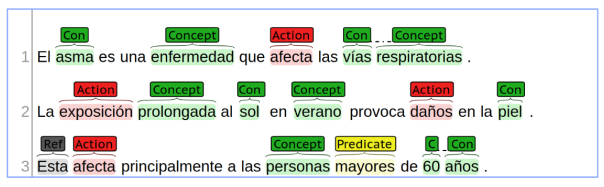
\includegraphics[width=0.9\linewidth]{Graphics/entities.png}
	\caption{Anotación de las entidades relevantes y sus respectivas clases en un conjunto de oraciones de ejemplo.} \label{fig:entites_ex}
\end{figure}

\begin{figure}[h!]
	\centering
	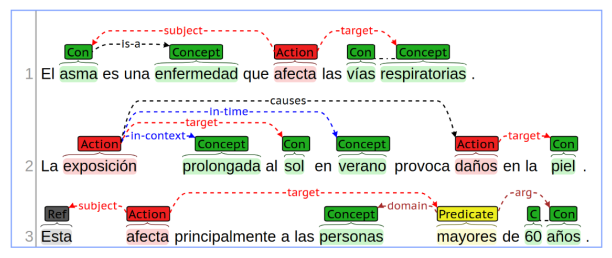
\includegraphics[width=0.9\linewidth]{Graphics/relations.png}
	\caption{Anotación de las relaciones semánticas relevantes en un conjunto de oraciones de ejemplo.} \label{fig:relations_ex}
\end{figure}


\subsection{Escenarios de Evaluación}\label{subsec:eval_sce}

El concurso propone un escenario de evaluación principal (Escenario 1) donde las dos tareas descritas anteriormente se realizan de forma secuencial.
Adicionalmente, los participantes tuvieron la oportunidad de enfocarse en una de las dos tareas específicamente, a partir de entregar resultados en dos escenarios opcionales, uno para cada tarea.
Estos dos escenarios adicionales miden el rendimiento en tareas individuales de forma independiente entre ellas.

\begin{description}
	
\item[Escenario 1 [A+B]:] Recibe como entrada un conjunto de oraciones a anotar.
El sistema produce tanto las instancias concretas de entidades
presentes en la colección como las relaciones existentes entre ellas.
El rendimiento general del sistema se mide en función
del rendimiento en ambas tareas, según se describe en la sección 4.1.2.
 
\item[Escenario 2 [A]:] Recibe como entrada un conjunto de oraciones a anotar.
El sistema produce únicamente el conjunto de entidades presentes en la colección (con la correspondiente clasificación según el tipo de concepto que representa).

\item[Escenario 3 [B]:] Recibe como entrada un conjunto de oraciones y una colección de entidades anotadas y etiquetadas en el texto.
El sistema produce únicamente el conjunto de relaciones que existen entre las instancias concretas de los conceptos.

\item[Escenario 4 [A+B~(Dominio General)]:] Este escenario fue incluido como una novedad en el evento del año 2020.
Es similar al Escenario 1 de evaluación, pero considera oraciones cuyo contenido es de dominio general.

\end{description}

\subsection{Métricas de Evaluación}

La métrica de evaluación es la medida \textit{F1} estándar, donde la precisión y recobrado se definen en términos de coincidencias \textbf{[C]orrectas}, \textbf{[I]ncorrectas},
\textbf{[P]arciales}, \textbf{[F]altantes} y \textbf{[S]obrantes}.


\begin{description}
	
	\item[Anotación correcta:] Reportada cuando una palabra clave es encontrada cuya sección de texto (secuencia de tuplas \texttt{<INICIO, FIN>}) coincide	exactamente con la de una en el corpus de referencia.
	Solo una coincidencia correcta por entrada en la colección de referencia puede ser reportada.
	Por tanto, las entradas duplicadas cuentan como Sobrantes.
	
	\item[Anotación incorrecta:] Reportada cuando una entidad es identificada correctamente en lo que a sección de texto respecta, pero no le fue asignado el tipo de concepto correcto.
	
	\item[Anotación parcial:] Reportada cuando dos intervalos \texttt{<INICIO, FIN>} tienen una intersección no vacía, como es el caso de “vías respiratorias”	y “respiratorias”.
	Notar que una anotación parcial es considerada solo sobre una única anotación correcta en la colección de referencia.
	
	\item[Anotación faltante:] Aquellas anotaciones que aparecen en la colección de	referencia pero no en la respuesta.
	
	\item[Anotación sobrante:] Aquellas anotaciones que aparecen en la respuesta pero no en la colección de referencia.
	
\end{description}

A las coincidencias parciales se les asigna la mitad de la
puntuaciones de las coincidencias correctas, mientras que a las anotaciones faltantes y sobrantes no se les da puntos.
Las fórmulas de evaluación para el Escenario 1 se definen de la siguiente forma:

\begin{equation*}
P = \frac{C_A + \frac{1}{2}P_A + C_B}{C_A + I_A + P_A + S_A + C_B + S_B}
\end{equation*}

\begin{equation*}
R = \frac{C_A + \frac{1}{2}P_A + C_B}{C_A + I_A + P_A + F_A + C_B + F_B}
\end{equation*}

\begin{equation*}
F1 = 2\frac{PR}{P+R}
\end{equation*}

Siendo $P$ y $R$ los valores de precisión y recobrado respectivamente.

Análogamente, se definen fórmulas similares para los escenarios 2 y 3, pero usando solo las estadísticas de la tarea A y B, respectivamente.

\subsection{Corpus de Evaluación}


\subsection{Implementación y Bibliotecas Externas}

La implementación de las propuestas se realizó utilizando el lenguaje de programación Python.
Se utilizó la biblioteca \texttt{PyTorch} como marco para el trabajo con redes neuronales profundas.
Para la obtención de los \textit{embedding} contextuales se utilizó una variente del modelo \texttt{BERT}~\cite{devlin2018bert}, en este caso: \texttt{bert-base-multilingual-uncased}, a través de la interfaz que brinda la biblioteca \texttt{pytorch-pretrained-bert}~\footnote{https://pypi.org/project/pytorch-pretrained-bert/}.
Los \textit{embeddings} de palabras fueron entrenados utilizado el algoritmo \texttt{word2vec}~\cite{mikolov2013efficient} con la arquitectura \texttt{skipgram}, utilizando la interfaz de la biblioteca \texttt{gensim}~\footnote{https://pypi.org/project/gensim/}.
Las etiquetas de POS-tag así como el árbol de dependencias fueron obtenidos utilizando la biblioteca \texttt{spaCy}~\footnote{https://spacy.io/}.

\subsection{Infraestructura Computacional}



\subsection{Entrenamiento y Ajuste de Parámetros}\label{sec:training}

Los algoritmos definidos para la resolución de ambas tareas, están basados en técnicas de aprendizaje profundo.
Una de las implicaciones de esta decisión, es que una vez fijo el algoritmo, existe una amplia variedad de hiperparámetros que se pueden ajustar en virtud de obtener mejores resultados computacionales.

Las tablas \ref{table:params_taskA} y \ref{table:params_taskB} describen las configuraciones de parámetros utilizadas cada uno de los modelos y para su entrenamiento.

\begin{table*}[tb]\centering
		\begin{tabular}{lc}
			\hline
			\textbf{Parámetro} & \textbf{Valor} \\
			\hline
			\hline
			\multicolumn{2}{c}{\textbf{Entradas}}\\
			\hline
			\hline
			Dim. del \textit{embedding} contextual & 9216~(12 capas)\\
			Dim. del \textit{embedding} de palabras & 300\\
			Dim. del \textit{embedding} de caracteres & 100\\
			Dim. del \textit{embedding} de POS-tag & 100\\
			
			\hline
			\hline
			\multicolumn{2}{c}{\textbf{Red neuronal}}\\
			\hline
			\hline
			
			Dimensión de la BiLSTM & 300\\
			
			\hline
			\hline
			\multicolumn{2}{c}{\textbf{Entrenamiento}}\\
			\hline
			\hline
			
			Optimizador & Adam\\
			\textit{Learning rate} & 0.001\\
			Épocas & 20\\
			
			\hline
			\hline
			
			\textbf{Total de parámetros} & X\\
			
			\hline
			
		\end{tabular}
	
	\caption{Configuración de parámetros del modelo de extracción de entidades. \textbf{[Arriba]} Red neuronal. \textbf{[Abajo]} Entrenamiento.}\label{table:params_taskA}
	
\end{table*}

\begin{table*}[tb]\centering
	\begin{tabular}{lc}
		\hline
		\textbf{Parámetro} & \textbf{Valor} \\
		\hline
		\hline
		\multicolumn{2}{c}{\textbf{Entradas}}\\
		\hline
		\hline
		Dim. del \textit{embedding} contextual & 768~(última capa)\\
		Dim. del \textit{embedding} de palabras & 300\\
		Dim. del \textit{embedding} de caracteres & 50\\
		Dim. del \textit{embedding} de POS-tag & 50\\
		Dim. del \textit{embedding} de dependencias & 50\\
		Dim. del \textit{embedding} de las etiquetas BMEWO-V & 50\\
		Dim. del \textit{embedding} del tipo de entidad & 50\\
		
		\hline
		\hline
		\multicolumn{2}{c}{\textbf{Red neuronal}}\\
		\hline
		\hline
		
		Dimensión de la BiLSTM & 100\\
		Dimensión de la Tree-LSTM & 50\\
		
		\hline
		\hline
		\multicolumn{2}{c}{\textbf{Entrenamiento}}\\
		\hline
		\hline
		
		Optimizador & Adam\\
		\textit{Learning rate} & 0.001\\
		Épocas & 30\\
		Muestreo negativo & 300\% de ej. positivos\\
		
		\hline
		\hline
		
		\textbf{Total de parámetros} & X\\
		
		\hline
		
	\end{tabular}
	
	\caption{Configuración de parámetros del modelo de extracción de relaciones. \textbf{[Arriba]} Red neuronal. \textbf{[Abajo]} Entrenamiento.}\label{table:params_taskB}
	
\end{table*}
		
Fueron entrenados modelos para ser evaluados tanto en el contexto del evento \textit{eHealth-KD} 2019, como en la edición del presente año.
En cada caso, la optimización de los modelos se realizó utilizando la colección de entrenamiento proveída a los concursantes.
El entrenamiento fue acompañado de un procedimiento de validación cruzada, que permitió determinar un número conveniente de épocas de entrenamiento, ajustar la complejidad de los modelos, así como seleccionar los más efectivos para someterlos a evaluación; para lo cual se utilizó la respectiva colección de desarrollo.


\section{Resultados Computacionales}

Los modelos fueron evaluados en los distintos escenarios de los eventos \textit{eHealth-KD} 2019 y en su edición del 2020.
Las tablas  \ref{table:results_19} y \ref{table:results_20} resumen el desempeño de todas propuestas participantes en los distintos escenarios de ambos eventos seg\'un la medida \emph{F1}. 

\begin{table*}[tb!]\centering
	\caption{Resultados (medida $F_1$) en cada escenario, ordenados por el Escenario 1 en el evento \textit{eHealth-KD} 2019. \label{table:results_19}}
	\begin{tabular}{|c|c|c|c|}
		\hline
		&  \multicolumn{2}{c|}{\textbf{Score($F_1$)}} \\
		\hline
		\textbf{Equipo} & \textbf{Escenario 1 (A+B)} & \textbf{Escenario 2 (A)} & \textbf{Escenario 3 (B)} \\
		\hline
		TALP	          	   &  0.6394 &  0.8203 &  0.6269 \\
		coin\_flipper (ncatala) & 0.6218 &  0.7873 &  0.4933 \\	
		LASTUS-TALN (abravo)   & 0.5816 &  0.8167 &  0.2298	\\
		NLP\_UNED               & 0.5473 &  0.7543 &  0.5337 \\
		Hulat-TaskAB           & 0.5413 &  0.7758 &  0.1231 \\	
		\textbf{UH-MAJA-KD}    & \textbf{0.5189} &  \textbf{0.8156} &  \textbf{0.4336} \\	
		lsi2\_uned              & 0.4934 &  0.7315 &  0.1231	\\
		IxaMed                 & 0.4869 &  0.6825 &  0.4356 \\
		baseline               & 0.4309 &  0.5466 &  0.1231 \\
		Hulat-TaskA            & 0.4309 &  0.7903 &  0.1231 \\	
		VSP             	   & 0.4289 &  0.5466 &  0.4933 \\	
		\hline
	\end{tabular}
\end{table*}

\begin{table*}[tb!]\centering
	\caption{Resultados (medida $F_1$) en cada escenario, ordenados por el Escenario 1 en el evento \textit{eHealth-KD} 2020. \label{table:results_19}}
	\begin{tabular}{|c|c|c|c|c|}
		\hline
		&  \multicolumn{2}{c|}{\textbf{Score($F_1$)}} \\
		\hline
		\textbf{Equipo} & \textbf{Escenario 1 (A+B)} & \textbf{Escenario 2 (A)} & \textbf{Escenario 3 (B)} &  \textbf{Escenario 4 (A+B)}\\
		\hline
		Vicomtech & 0.6655 & 0.8208 & 0.5832 & 0.5632 \\
		Talp-UPC & 0.6266 & 0.8158 & 0.5747 & 0.5835  \\
		\textbf{UH-MAJA-KD} & \textbf{0.6250} & \textbf{0.8143} & \textbf{0.5987} & \textbf{0.5477} \\
		IXA-NER-RE & 0.5574 & 0.6918 & 0.633235 & 0.4788 \\
		UH-MatCom &	0.5568 & 0.7949 & 0.5450 & 0.37307 \\
		SINAI &	0.4206 & 0.8252 & 0.4617 & 0.28125 \\
		HAPLAP & 0.3951 & 0.5419 & 0.3164 & 0.1377 \\
		baseline & 0.3951 & 0.5419 & 0.1313 & 0.1377 \\
		ExSim &	0.2456 & 0.3142 & 0.1313 & 0.1222 \\
		\hline
	\end{tabular}
\end{table*}


\subsection{Resultados por Escenarios de Evaluación}

A continuación se profundiza en el desempeño de la propuesta en los escenarios, no solo en términos de medida $F1$, sino también de precisión y recobrado.
Las tablas \ref{table:sce_19} y \ref{table:sce_20} resumen los resultados obtenidos en los eventos correspondientes a cada año, respectivamente.

Como se puede observar en la tabla~\ref{table:sce_19}, el sistema presentado obtiene el primer lugar en el Escenario 1 (A + B) con una ligera diferencia con respecto al segundo mejor sistema. Cuando se comparan los resultados presentados en la tabla~\ref{table:sce_20}, el modelo obtiene el tercer lugar en la competencia en el Escenario 1 (A + B) con una diferencia de 0.001 aproximadamente con respecto al segundo lugar, lo cual significa que solo el sistema en primer lugar supera considerablemente al modelo presentado.

En la tabla(PONER REF) se aprecian los resultados m\'as detallados del Escenario 2 (A) en el evento del 2019. Se puede notar que el modelo presentado para resolver la \emph{Tarea} A supera a todos los modelos presentados, obteniendo el primer lugar en dicha tarea. En cuanto a los resultados en el mismo escenario en el evento del 2020, presentados en la tabla(PONER REF), se puede apreciar que aunque se posiciona en cuarto lugar, el modelo obtiene resultados competitivos con respecto a los primeros tres lugares, donde los resultados de las primeras 4 posiciones son muy similares existiendo una diferencia que no supera el 2\%.

(PONER LOS RESPECTIVOS A LOS ESCENARIOS DE RELACIONES)
 
(Tablas, muchas tablas)

(Muela de las tablas)

\subsection{Curvas de Aprendizaje}

Se analizaron las curvas de aprendizaje para medir el impacto que tiene en la efectividad de los modelos el tamaño del conjunto de datos utilizado.
Los gráficos \ref{plot:learning_curves_ent} y \ref{plot:learning_curves_rel} muestran los resultados de entrenar con conjuntos de datos de distintos tamaños los modelos de entidades y relaciones respectivamente.
Los experimentos se realizaron utilizando las colecciones de entrenamiento y desarrollo del evento correspondiente al año 2020.

(Graficos, muchas graficos)

(Muela de los graficos)

\subsection{Análisis Ablasivo}

Con el objetivo de medir la influencia de las representaciones distribuidas empleadas, se realizó un análisis ablasivo sobre las distintas componentes de la entrada de los modelos.
Las tablas \ref{table:ablation_ent} y \ref{table:ablation_rel} resumen el desempeño de las distintas configuraciones consideradas.
Los experimentos fueron realizados utilizando los datos del evento correspondiente al año 2020.

(Tablas, muchas tablas)

(Muela de las tablas)

\subsection{Hipótesis del Árbol de Dependencias}

En el caso del modelo para la extracción de relaciones, se evaluaron adicionalmente las hipótesis sobre el árbol de dependencias.
Para ello se entrenó un modelo con una complejidad semejante en términos de parámetros.
Se sustiuyó el camino en el árbol de dependencias por la secuencia de palabras de la oración completa, y se cambió el procesamiento mediante Tree-LSTM del subárbol relevante a las entidades, por una codificación basada en BiLSTM de las palabras que forman parte de las mismas.
Este modelo tiene un total de X parámetros, cifra cercana a los Y parámetros del modelo basado en estructuras de dependencias.

La tabla \ref{table:dep_cmp} muestra una comparación del desempeño de las dos variantes, en el entorno del evento correspondiente al año 2020. Se incluyen los resultados obtenidos por otros participantes como referencia.

(Tablas, muchas tablas)

(Muela de las tablas)


\section{Discusión}
%================
El modelo presentado obtuvo resultados relevantes en los contextos de ambos eventos del \emph{eHealth-KD Challenge} (2019 y 2020). Esto constituye un m\'erito de por si, pues muestra resultados cercanos al estado del arte en el evento (PONER NOMBRE DEL EVENTO). Este sistema supera por completo al presentado anteriormente en la competencia del 2019(PONER REF) e incluso obtiene mejores resultados que el mejor sistema en dicha comptencia, el cual resuelve las tareas A y B en un \'unico sistema \emph{end-to-end}. Es natural pensar que un sistema que resuelva ambas tareas a la vez obtendr\'a mejor rendimiento en general, pues existe una estrecha interrelaci\'on entre ambas tareas, sin embargo el modelo presentado las resuelve por separado y obtiene resultados muy similares, lo que sugiere que un modelo que resuelva ambas tareas haciendo uso de las caracteristicas esenciales de los modelos presentados para resolver las tareas A y B respectivamente pueda obtener un mejor desempe~no y avanzar el estado del arte.

Particularmente en el escenario 2 se puede apreciar como el sistema posee muy buenos resultados, siendo el mejor en el contexto de la competencia del 2019 y teniendo resultados competitivos en el 2020. El modelo presentado para resolver la Tarea A sugiere varios aspectos interesantes. En primer lugar, como se pudo observar a trav\'es de la experimentaci\'on, los embeddings contextuales para cada palabra construidos a partir del modelo preentrenado de \textbf{BERT} son rasgos de gran impacto en la resoluci\'on de la Tarea A(PONER REF AL ANALISIS ABLASIVO). A partir del an\'alisis ablasivo se puede notar como cada una de los features que forman parte de la entrada tienen importancia para obtener el mejor desempe~no. A pesar de que el modelo de \textbf{BERT} fue entrenado de forma bidireccional en un gran corpus con m\'ultiples lenguajes, a\'un asi no ha sido entrenado necesariamente en las oraciones que conforman el corpus del evento, por lo que los embeddings contextuales obtenidos de \textbf{BERT} no obtienen los mejores resultados, a pesar de contener mucha informaci\'on como se pudo apreciar en el experimento haciendo uso solamente del modelo preentrenado de \textbf{BERT} y las capas de \textbf{CRF} a\'un as\'i el uso de rasgos como los embeddings de caracteres y los embeddings de PosTag, mejoran el desempe\~no del sistema. De la misma forma a partir de las \emph{Stacked BiLSTM} se construyen embeddings contextuales que contienen m\'as informacion, pues adem\'as de hacer uso de los embeddings contextuales preentrenados con \textbf{BERT}, hace uso de los character embeddings y PosTag embeddings analizando la oraci\'on bidireccionalmente obteniendo mayor informaci\'on para cada palabra dependiente del contexto y consiguiendo a\'un m\'as complejos rasgos dependientes del contexto con la segunda \emph{BiLSTM}. Otra observaci\'on interesante durante la experimentaci\'on es que como se ha visto en el estado del arte el uso de Embeddings de Palabras para la representaci\'on de las mismas y contruir embeddings contextuales a partir de estas ha obtenido muy buenos resultados en muchos trabajos(PONER REF), pero a\'un as\'i los experimentos utilizando los embeddings contextuales preentrenados a partir de \textbf{BERT} en lugar de los Embeddings de Palabras obtienen mejores resultados que los experimentos realizados con los Embeddings de Palabras y combinando los embeddings contextuales de \textbf{BERT} con los Embeddings de Palabra(PENSAR EN COMO EXPLICAR ESTO).








===================================================================